\section{Evaluation}

\label{sec:evaluation}

To evaluate our strategy, in this section we present the empirical study we conduct. The objective of this study is to evaluate to what extent our strategy is capable of identifying potential failing students in only 30 days. To explain our evaluation design, we first present the participants and material in Section~\ref{sec:participants}. Then, we detail the procedure we use during the evaluation in Section~\ref{sec:procedure}.

%Before explaining our study, we first introduce the terminology we use throughout this paper. In particular, we define in what follows four categories: abort, skip, fail, and pass.
%
%\begin{itemize}
%
%	\item \textbf{Abort:} students that aborted the course before the final exam;
%	\item \textbf{Skip:} students allowed to do the final exam but did not show up;
%	\item \textbf{Fail:} students who failed the course;
%	\item \textbf{Pass:} students who successfully passed the course.
%
%\end{itemize}

%Now, we present the objetives and hypothesis (Section~\ref{sec:hypotheses}) of our study, then the participants and material (Section~\ref{sec:participants}) we use, and finally we detail the procedure (Section~\ref{sec:procedure}) we use during the evaluation.

%\subsection{Objective and Hypothesis}

%\label{sec:hypotheses}

%The objective of this study is to evaluate to what extent our strategy is capable of identifying potential failing students. This way, based on this objective, our hypothesis is the following: In the first 30 days, students with lower number of submissions and correct submissions tend to fail the course.

\subsection{Participants and Material}

\label{sec:participants}

The participants of our study are students of introductory programming courses at the Federal University of Alagoas, Brazil. We ministered these courses during 3.5 years and collected the metrics we detail in Section~\ref{sec:metrics} of each student by using Huxley. The professor encouraged all students to use Huxley to practice by solving the available problems. The use of Huxley was mandatory only during formal exams. Table~\ref{tab:participants} distribute the number of participants per semester.

\begin{table}[h]
\centering
\begin{tabular}{|c|c|}
\hline
\textbf{Course} & \textbf{Number of enrolled students}\\ \hline
2010.02 & 32\\ \hline
2011.01 & 38\\ \hline
2011.02 & 35\\ \hline
2012.01 & 34\\ \hline
2012.02 & 29\\ \hline
2013.01 & 28\\ \hline
2013.02 & 31\\ \hline
\textbf{TOTAL:} & \totalStudents\\ \hline
\end{tabular}
\caption{Participants per course.}
\label{tab:participants}
\end{table}

The material of this study consists of almost 300 programming exercises in Huxley. They were available for all students of all courses we use in this paper.

\subsection{Procedure}

\label{sec:procedure}

Figure~\ref{fig:procedure} illustrates how we perform our evaluation. The result of executing our strategy consists of groups of students according to the clustering algorithm. Now, according to the groups, we have the potential failing students (see the left-hand side in Figure~\ref{fig:procedure}). These students are the ones that have a small number of submissions and correct submissions (represented by circles). Notice we also have students that are potential candidates to successfully pass (represented by stars): due to the high number of submissions to Huxley after 30 days, they seem to be practicing programming really hard. We represent the inconclusive group by squares.

\begin{figure}[htb]
\centering
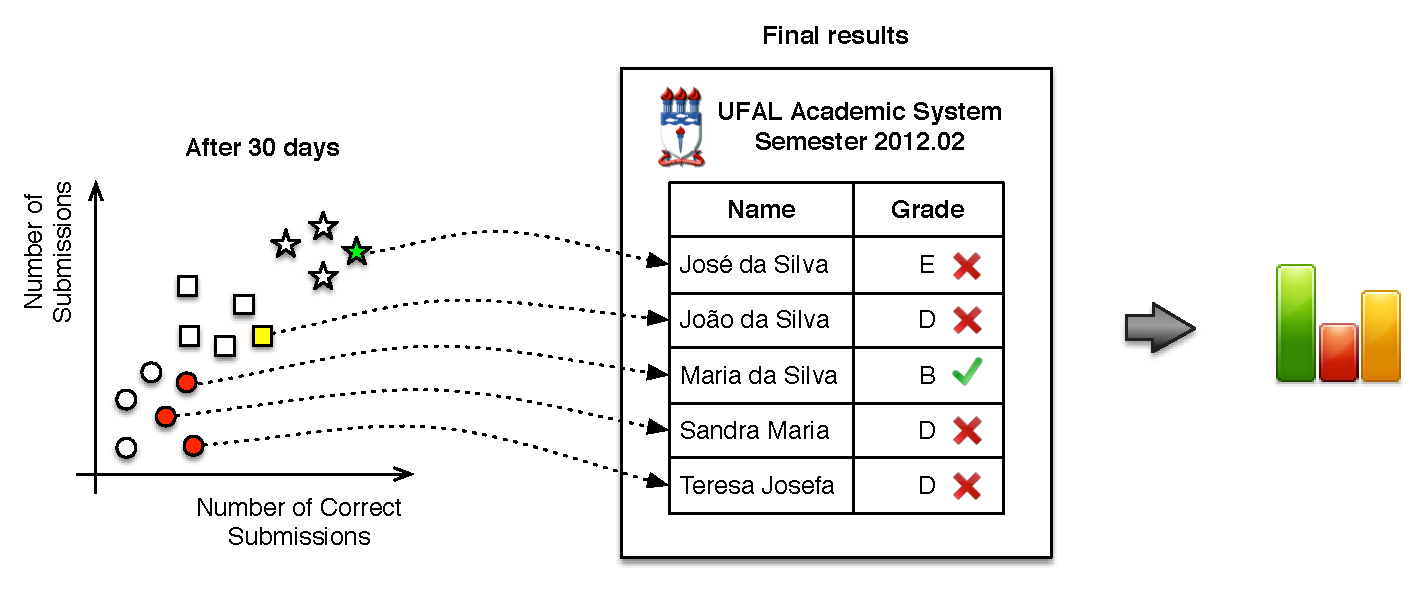
\includegraphics[width=1.0\textwidth,natwidth=950,natheight=394]{images/Procedure.pdf}
\caption{Checking the strategy results against the actual grades.}
\label{fig:procedure}
\end{figure}

After applying the strategy, we now need to check whether it correctly predicts the failing students after 30 days. To do so, we use the academic system of the Federal University of Alagoas to look for grades and check whether the students failed or not. For example, for the detached circles, the strategy successfully identified that, after 30 days, two students would not pass and they indeed did not. Notice, however, that we may face false positives. Despite indicating the student \textit{Maria da Silva}\footnote{All names we consider in this paper are fictitious.} as a failing one after 30 days, such a student seemed to improve herself during the semester and she has been approved. In addition, we may also have false negatives. For instance, our strategy does not point the students \textit{Jos\'{e} da Silva} and \textit{Jo\~{a}o da Silva} as failing ones. Although \textit{Jos\'{e} da Silva} seems to be one of the best students after 30 days, he failed the course. The several reasons why this happened is out of the scope of this paper.

To better structure and analyze our results and, at the same time, take false positives and false negatives into account, we consider the following two metrics: precision and recall. Precision is the fraction of retrieved students that are relevant, i.e., the students pointed by the strategy that indeed failed the course. We have a perfect precision, 1.0, when every student retrieved by the strategy is relevant (i.e., a failing student), which means we have no false positives. Precision focuses on \textit{quality} and \textit{accuracy}. However, the precision says nothing about whether \textit{all} relevant students were indeed retrieved.

\vspace{0.1cm}
$$
Precision = \frac{| \{relevant\_students\} \cap \{retrieved\_students\} |}{| \{retrieved\_students\} |}
$$
\vspace{0.1cm}

Recall, in its turn, is the fraction of relevant students that are retrieved, i.e., it is the probability of retrieving a failing student. A perfect recall, 1.0, means that we retrieve all failing students, which means we have no false negatives. In this context, recall focuses on \textit{completeness} and \textit{quantity}. Notice that recall says nothing about how many irrelevant students (students that will pass) the strategy retrieved.

\vspace{0.1cm}
$$
Recall = \frac{| \{relevant\_students\} \cap \{retrieved\_students\} |}{| \{relevant\_students\} |}
$$
\vspace{0.1cm}

To better explain these metrics, consider the detached students in Figure~\ref{fig:procedure} as our set (three circles, one square, and one star). The relevant set is \textit{\{Jos\'{e}, Jo\~{a}o, Sandra, Teresa\}}, whereas the retrieved set is \textit{\{Maria, Sandra, Teresa\}}. The intersection set is \textit{\{Sandra, Teresa\}}. This way, we have

\vspace{0.2cm}
\noindent
\scriptsize
\begin{minipage}{.5\linewidth}
\centering
$$
Precision = \frac{|\{Sandra, Teresa\}|}{|\{Maria, Sandra, Teresa\}|} = 67\%;
$$
\end{minipage}
\begin{minipage}{.5\linewidth}
$$
Recall = \frac{|\{Sandra, Teresa\}|}{|\{\textit{\text{Jos\'{e}}}, \textit{\text{Jo\~{a}o}}, Sandra, Teresa\}|} = 50\%.
$$
\end{minipage}
\normalsize
\vspace{0.2cm}

Our strategy pointed two out of three students as failed ones and they indeed failed. Therefore, we have 67\% of accuracy when identifying potential failing students, raising one false positive. On the other hand, only two out of four students have been pointed as failed ones. This means that the strategy was not able to identify all failing students, raising two false negatives.

Last but not least, after confronting the strategy results with the academic system and summarizing precision and recall, we apply a statistical test to check for significance. Here, we rely on the proportion statistical test based on the Bernoulli distribution~\cite{} so that we have a binary distribution: fail or pass. In this paper, we follow the convention of considering a factor as being significant to the response variable when \textit{p-value} $< 0.05$~\cite{}.

\section{Results and Discussion}

In this section, we describe the results and test our hypotheses before discussing their implications. All data, materials, and R scripts are available at \url{http://www.ic.ufal.br/}.

\subsection{Results}

In our evaluation, we use data of 7 courses (3.5 years) totalling \totalStudents students. We apply our strategy by setting k-means to compute two and three groups. We now proceed separately, reporting the results considering both cases.

\subsubsection{Two groups}

When considering two groups, we set the strategy to consider all students in two categories: fail or pass. Figure~\ref{fig:2-groups} illustrates the results for all courses. Notice that Figure~\ref{fig:2-2011-01} contains an outlier. In this particular case, the strategy pointed that all students but one would fail the course. Clearly this result is a consequence of such outlier. This way, the presence of one outlier might represent a problem when considering two groups.

\begin{figure*}[ht]
     \begin{center}
         \subfigure[2010.02] {
             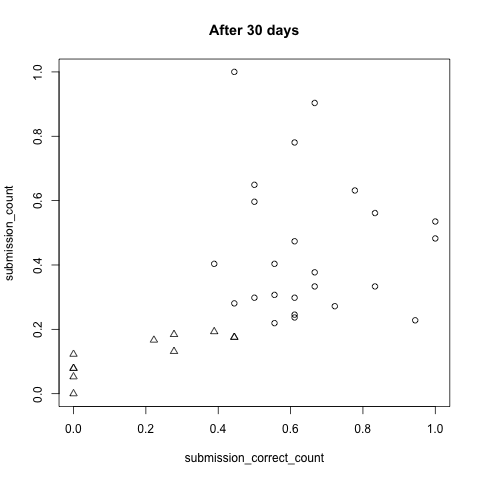
\includegraphics[scale=0.21,natwidth=480,natheight=480]{images/2-2010-02.png}
             \label{fig:2-2010-02}
         }
         \subfigure[2011.01] {
             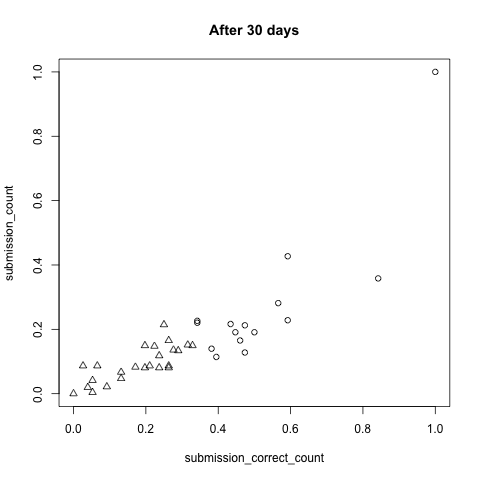
\includegraphics[scale=0.21,natwidth=480,natheight=480]{images/2-2011-01.png}
             \label{fig:2-2011-01}
         }
         \subfigure[2011.02] {
             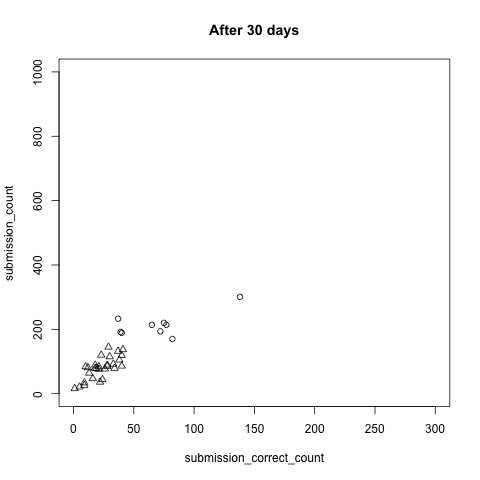
\includegraphics[scale=0.21,natwidth=480,natheight=480]{images/2-2011-02.png}
             \label{fig:2-2011-02}
         }
         \subfigure[2012.01] {
             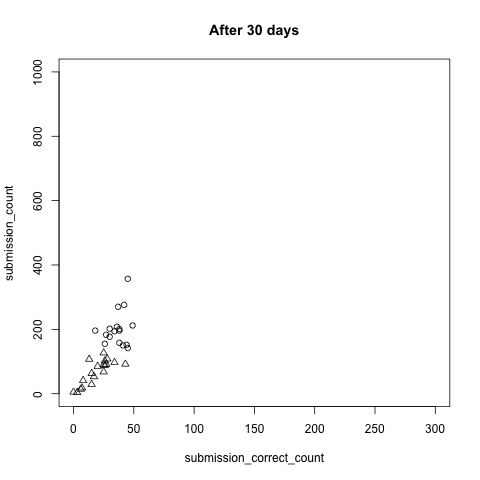
\includegraphics[scale=0.21,natwidth=480,natheight=480]{images/2-2012-01.png}
             \label{fig:2-2012-01}
         }
         \subfigure[2012.02] {
             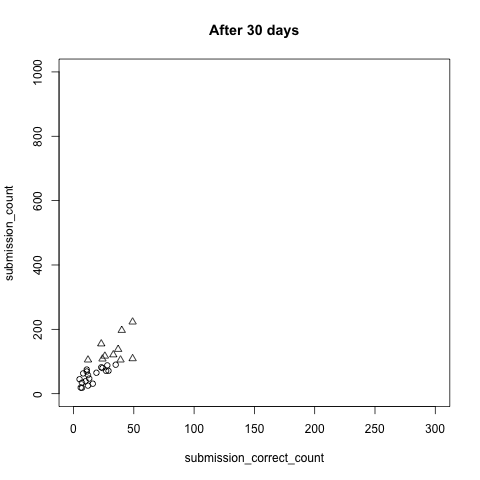
\includegraphics[scale=0.21,natwidth=480,natheight=480]{images/2-2012-02.png}
             \label{fig:2-2012-02}
         }
         \subfigure[2013.01] {
             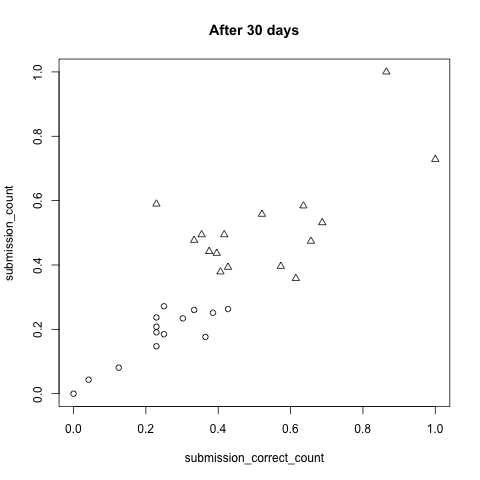
\includegraphics[scale=0.21,natwidth=480,natheight=480]{images/2-2013-01.png}
             \label{fig:2-2013-01}
         }
         \subfigure[2013.02] {
             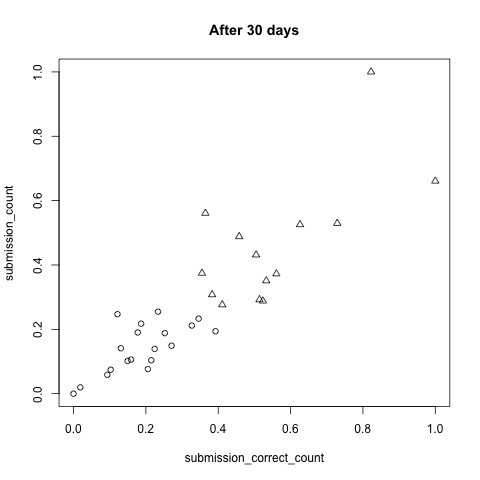
\includegraphics[scale=0.21,natwidth=480,natheight=480]{images/2-2013-02.png}
             \label{fig:2-2013-02}
         }
     \end{center}
     \caption{Strategy applied with two groups.}
	 \label{fig:2-groups}
\end{figure*}

To better analyze our results, we remove this outlier and execute our strategy again. By using two groups and properly removing the outlier, we achieve the following results for precision and recall:

\vspace{0.2cm}
\noindent
\begin{minipage}{.5\linewidth}
\centering
$$
Precision = \frac{92}{145} = 63\%;
$$
\end{minipage}
\begin{minipage}{.5\linewidth}
$$
Recall = \frac{92}{115} = 80\%.
$$
\end{minipage}
\vspace{0.2cm}

Here we observe a high recall, i.e., 80\%. This means we only miss 20\% of the failing students. We have few false negatives, but this result says nothing about how many false positives (irrelevant students) we retrieved. Notice that this result (80\%) represents our particular sample. We now need to find the population proportion, enabling us to generalize our findings. To do so, we need to check for statistical significance by executing the proportion hypothesis test. In this context, the test reveals that the population recall is 73\% with a confidence level of 95\% (\textit{p-value} $= 0.045$). Regarding precision, our results show a sample precision of 63\%. To generalize, we again execute the test and find that the population precision would be 56\% (\textit{p-value} $= 0.035$).

\subsubsection{Three groups}

Analogously, we set our strategy to consider three groups. Here, besides the failing and passing groups, there is one extra group where the strategy cannot conclude anything about it. Figure~\ref{fig:3-groups} shows the results for three groups. Differently from two groups, here one outlier does not completely compromise the strategy.

\begin{figure*}[ht]
     \begin{center}
         \subfigure[2010.02] {
             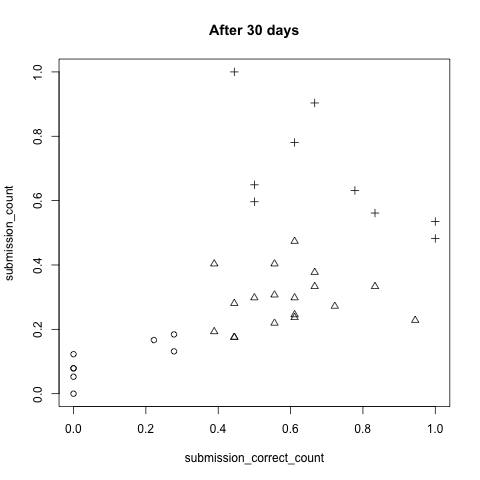
\includegraphics[scale=0.21,natwidth=480,natheight=480]{images/3-2010-02.png}
             \label{fig:3-2010-02}
         }
         \subfigure[2011.01] {
             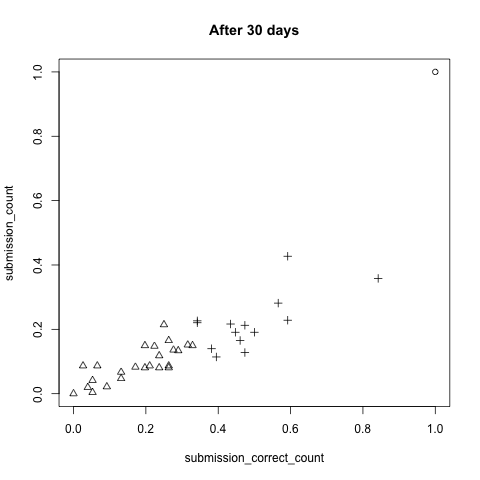
\includegraphics[scale=0.21,natwidth=480,natheight=480]{images/3-2011-01.png}
             \label{fig:3-2011-01}
         }\\
         \subfigure[2011.02] {
             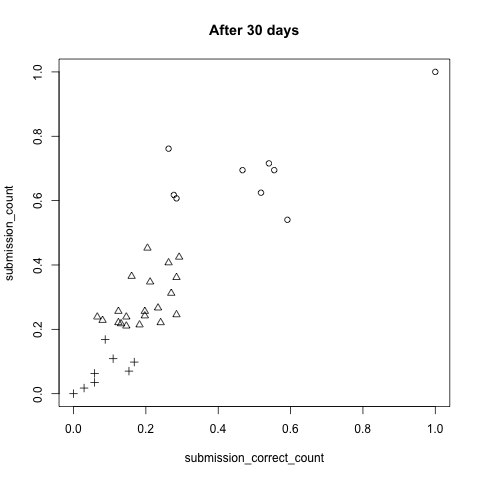
\includegraphics[scale=0.21,natwidth=480,natheight=480]{images/3-2011-02.png}
             \label{fig:3-2011-02}
         }
         \subfigure[2012.01] {
             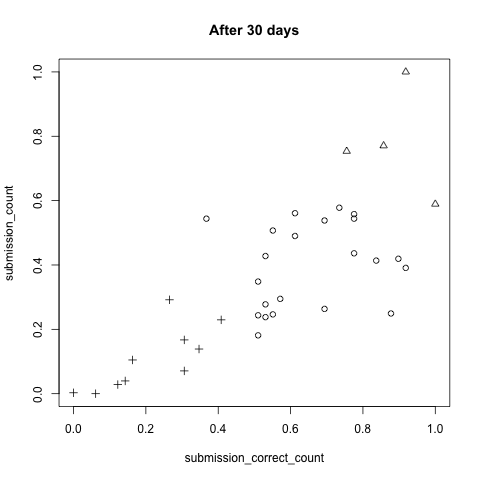
\includegraphics[scale=0.21,natwidth=480,natheight=480]{images/3-2012-01.png}
             \label{fig:3-2012-01}
         }\\
         \subfigure[2012.02] {
             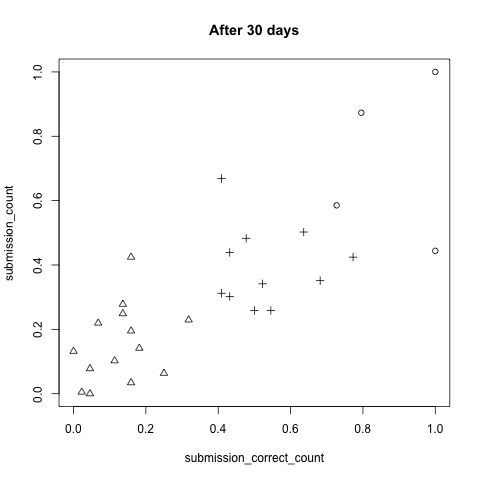
\includegraphics[scale=0.21,natwidth=480,natheight=480]{images/3-2012-02.png}
             \label{fig:3-2012-02}
         }
         \subfigure[2013.01] {
             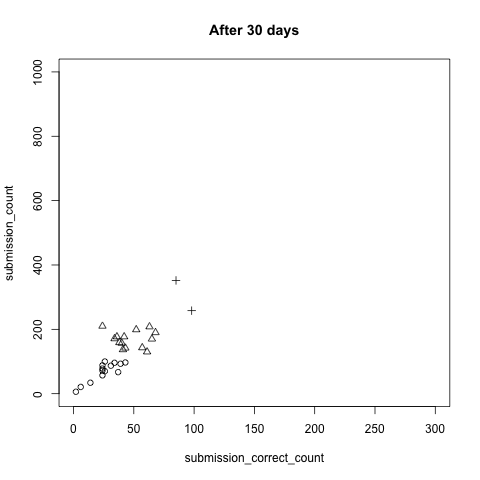
\includegraphics[scale=0.21,natwidth=480,natheight=480]{images/3-2013-01.png}
             \label{fig:3-2013-01}
         }\\
         \subfigure[2013.02] {
             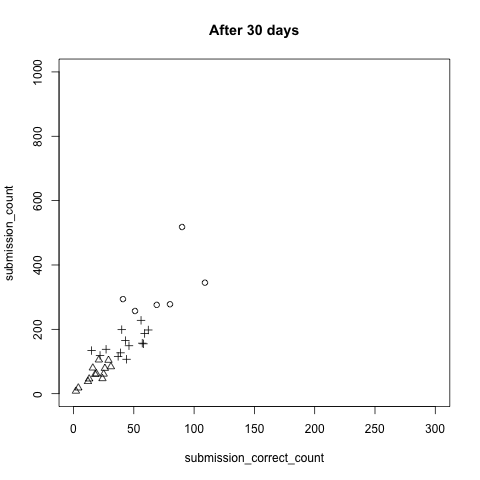
\includegraphics[scale=0.21,natwidth=480,natheight=480]{images/3-2013-02.png}
             \label{fig:3-2013-02}
         }
     \end{center}
     \caption{Strategy applied with three groups.}
	 \label{fig:3-groups}
\end{figure*}

We present the precision and recall for three groups in what follows:

\vspace{0.2cm}
\noindent
\begin{minipage}{.5\linewidth}
\centering
$$
Precision = \frac{73}{91} = 80\%;
$$
\end{minipage}
\begin{minipage}{.5\linewidth}
$$
Recall = \frac{73}{115} = 63\%.
$$
\end{minipage}
\vspace{0.2cm}

Now the strategy returns a precision of 80\% for the sample proportion. To generalize our results, we again execute the proportion hypothesis test. Regarding the population, our results reveal that the precision would be 72\% with a confidence level of 95\%. In other words, after 30 days, we can identify with statistical significance (\textit{p-value} $= 0.04$) 72\% of the students that indeed will fail the course. We repeat this process for recall and find 63\% for the sample and 55\% for the population, \textit{p-value} $= 0.033$.

Notice that with three groups the results of precision and recall are inverted when compared to two groups. Our strategy uses k-means, which takes into account two metrics---number of submissions and number of correct submissions---and the number of groups. Both executions are totally independent and the algorithm is not aware of precision, recall, and the academic system. Therefore, we take these results as a coincidence.

\subsection{Discussion}

In this section we discuss the results. We first discuss the number of groups

focus on the results for two groups and then we discuss the results for three groups.

\subsubsection{Two or Three Groups?}

When applying our strategy considering two groups, the results indicate a high recall. This means that the strategy can identify the majority of the failing students (raising only few false negatives). Although this is an interesting result, the strategy with two groups yields many false positives. In fact, the precision is low, i.e., the retrieved set contains many students that passed). In this situation, professors and assistants might waste effort trying to recover students that actually do not need recovering. On the other hand, with three groups we have a high precision, which means professors should give special attention to these students, since 72\% of them tend to fail. Nevertheless, since the recall is low, there are many failing students not retrieved by the strategy.

In this context, setting the number of groups to execute our strategy seems to depend on the professors priorities and resources. In case the professor has available time and additional assistants to help her, she can probably use two groups, which consists of a more complete retrieved set (the recall is high), even though it contains many false positives. However, it is important to notice that applying the strategy with two groups is more likely to outliers problems.

On the other hand, if the professor wants to avoid false positives because of situations like no available time or few assistants to help, she might prefer to use three groups, despite being aware of potential failing students not retrieved by the strategy (many false negatives, low recall). 

%better precision in exchange for 

\subsubsection{Final Exams}

Even though the strategy pointed students as potential failing ones in the first 30 days, some of them passed, raising false positives. Table~\ref{tab:final-exams} illustrates the precision for two and three groups as well as the false positives. For two and three groups, the precision is 56\% and 72\%, respectively. This way, we have 44\% and 28\% of false positives. As mentioned, the number of false positives is greater when considering two groups.

\begin{table}[h]
\centering
\begin{tabular}{|c|c|c|c|}
\hline
\textbf{Groups} & \textbf{Precision} & \textbf{False Positives} & \textbf{Final Exam}\\ \hline
2 & 56\% & 44\% (53 students) & 35\% (19 out of 53 students)\\ \hline
3 & 72\% & 28\% (18 students) & 33\% (06 out of 18 students)\\ \hline
\end{tabular}
\caption{False positives (students pointed as potential failing ones but passed) that performed the final exam.}
\label{tab:final-exams}
\end{table}

To better understand these false positives, we now analyze their grades at the academic system. In our study, we find that some of these students did not pass in the first place. In fact, they needed to perform the final exam to pass. At the university we focus on this paper, the final exam represents a second chance and is only available to students with not enough grades to pass.

This result is important in the sense that, although the strategy might raise false positives, it seems worth to follow these students as well. We find that at least 1/3 of them will need help (regardless of the number of groups, two or three), otherwise they reach the final exams. This way, professors and assistants can also give special attention to these students, which may improve their learning process, avoid final exams, and lead to better grades.

\subsubsection{Back to our objective}

As mentioned, the objective of our study is ``to evaluate to what extent our strategy is capable of identifying potential failing students in only 30 days.'' Given the results we achieve, we believe our strategy is indeed capable of identifying the failing students early. In particular, from the group of students our strategy points as ``likely to fail'' by using three groups, it hits 72\% of students that indeed fail with 95\% standard confidence level. Also, we notice that the 28\% remaining contains at least 33\% of students that somehow need help, since they reach the final exam.

\subsection{Threats to validity}

In this section we present the threats to validity of our study. Although our sample is reasonably big (227 students), our study has homogeneities that might pose threats. For example, the same professor for all the 7 courses and the same language used (C language) threats external validity. In this way, it is difficult to extrapolate the results to other contexts. Nevertheless, our strategy uses metrics to identify potential failing students. In this context, we argue that the metrics we use (submissions and correct submissions) do not necessarily depend on factors such as the professors and even less on the adopted languages. However, our claim is not enough and we need further studies to better generalize our conclusions.

The use of Huxley threats internal validity. Students must know how to use the system to submit their solutions. If the students somehow do not get used to the system, they might feel frustrated, hindering their learning and, consequently, biasing our results. We minimize this threat by introducing Huxley in the very first classes as well as by using assistants to help the students on how to use Huxley.